O capítulo atual irá desenvolver a arquitetura adotada para o uso de Blockchains e Hysail. Para a reestruturação da arquitetura já estabelecida
em Hysail, alguns aspectos já definidos serão modificados para a implementação do uso de Blockchains como meio de auditoria. A seguir, serão
apresentados os principais aspectos da nova arquitetura proposta.

\section{LtCode e OnlineCodes}

Os erasure codes desempenham um papel fundamental em sistemas distribuídos modernos, particularmente em ambientes blockchain e de armazenamento distribuído. Entre as várias famílias de erasure codes, os LtCodes (Luby Transform codes) e OnlineCodes representam duas abordagens distintas para o problema de recuperação de dados em cenários de falhas parciais.

\subsection{Definições e Características}

\textbf{LtCodes} pertencem à classe dos códigos fountain digitais (digital fountain codes), baseados na transformada de Luby, introduzidos por Michael Luby em 2002 \cite{luby2002lt}. Esses códigos são construídos randomicamente durante o processo de codificação, onde cada símbolo codificado é gerado através da combinação linear de um número variável de símbolos de origem. A distribuição de grau é otimizada para minimizar o número de símbolos necessários para a recuperação completa dos dados, adotando a distribuição de grau de Sóliton robusta (robust Soliton distribution), isto é, a distribuição de Sóliton ideal acrescida de um termo corretivo para elevar a probabilidade de decodificação completa com baixo overhead \cite{shokrollahi2006raptor}.

\textbf{OnlineCodes}, por sua vez, foram desenvolvidos para oferecer capacidades incrementais de codificação e decodificação \cite{peleg2004online}. Esses códigos permitem que o processo de codificação ocorra de forma contínua, com a possibilidade de gerar símbolos codificados indefinidamente, enquanto mantêm a garantia de recuperabilidade. A característica fundamental dos OnlineCodes é sua natureza online, permitindo processar dados conforme chegam, sem necessidade de acesso aleatório ou retorno aos dados anteriores.

\subsection{Robust Soliton Distribution}

Nos LtCodes, a escolha do grau de cada símbolo codificado é controlada pela robust Soliton distribution, proposta para melhorar o desempenho de decodificação em tamanho finito \cite{luby2002lt,karp2004finite}. A construção parte de duas distribuições: a distribuição de Soliton ideal $\rho(d)$ e um termo corretivo $\tau(d)$.

Para $k$ simbolos de origem, a distribuicao ideal e dada por:

\begin{equation}
\rho(d) = \begin{cases}
\frac{1}{k}, & d=1 \\
\frac{1}{d(d-1)}, & d=2,\ldots,k
\end{cases}
\end{equation}

Define-se $R = c\ln\left(\frac{k}{\delta}\right)\sqrt{k}$, com $c>0$ e $\delta \in (0,1)$. O termo corretivo é:

\begin{equation}
\tau(d) = \begin{cases}
\frac{R}{dk}, & d=1,\ldots,\left\lfloor\frac{k}{R}\right\rfloor-1 \\
\frac{R\ln\left(\frac{R}{\delta}\right)}{k}, & d=\left\lfloor\frac{k}{R}\right\rfloor \\
0, & d>\left\lfloor\frac{k}{R}\right\rfloor
\end{cases}
\end{equation}

A robust Soliton distribution final é a normalização:

\begin{equation}
\mu(d) = \frac{\rho(d)+\tau(d)}{Z}, \quad Z = \sum_{i=1}^{k} \left(\rho(i)+\tau(i)\right)
\end{equation}

Essa formulação aumenta a probabilidade de existência de símbolos de grau baixo durante a decodificação por \emph{belief propagation}, reduzindo o risco de estagnação do processo e mantendo baixo overhead de recepção \cite{luby2002lt,hyytia2007analysis}.

\subsection{Operações Matemáticas}

\subsubsection{LtCodes}

Os LtCodes utilizam operações XOR iterativas em corpos finitos (típicamente GF(2) para aplicações binárias). Seja $\mathbf{d} = (d_1, d_2, \ldots, d_k)$ o vetor 
contendo os $k$ símbolos de origem, o processo de codificação gera $n$ símbolos codificados $\mathbf{c} = (c_1, c_2, \ldots, c_n)$ conforme:

\begin{equation}
c_i = \bigoplus_{j \in S_i} d_j
\end{equation}

onde $\bigoplus$ denota a operação XOR (ou soma em GF(2)), e $S_i$ é um subconjunto de índices selecionados randomicamente de acordo com 
uma distribuição de grau Soliton. O grau $|S_i|$ segue uma distribuição de probabilidade específica $\rho(d)$:

\begin{equation}
\rho(d) = \begin{cases}
1/k & \text{se } d = 1 \\
1/(d(d-1)) & \text{se } d = 2, 3, \ldots, k
\end{cases}
\end{equation}

A decodificação procede iterativamente, identificando símbolos codificados com grau 1 (que correspondem diretamente a símbolos de origem) e propagando 
a informação até recuperar todos os $k$ símbolos originais. Este processo é denominado \emph{belief propagation}.

\subsubsection{OnlineCodes}

Os OnlineCodes utilizam um sistema de equações lineares sobre corpos finitos, mas com uma estrutura mais rígida. Dado um vetor de 
origem $\mathbf{d} = (d_1, d_2, \ldots, d_k)$, a codificação gera símbolos mediante:

\begin{equation}
c_i = \sum_{j=1}^{k} g_{i,j} \cdot d_j \pmod{p}
\end{equation}

onde $g_{i,j}$ são coeficientes determinados por uma função geradora pseudoaleatória, e $p$ é um número primo grande. Para cada símbolo 
codificado $c_i$, armazena-se também o vetor de coeficientes $\mathbf{g}_i = (g_{i,1}, g_{i,2}, \ldots, g_{i,k})$.

A decodificação resolvem um sistema linear:

\begin{equation}
\begin{pmatrix}
g_{1,1} & g_{1,2} & \cdots & g_{1,k} \\
g_{2,1} & g_{2,2} & \cdots & g_{2,k} \\
\vdots & \vdots & \ddots & \vdots \\
g_{m,1} & g_{m,2} & \cdots & g_{m,k}
\end{pmatrix}
\begin{pmatrix}
d_1 \\ d_2 \\ \vdots \\ d_k
\end{pmatrix}
=
\begin{pmatrix}
c_1 \\ c_2 \\ \vdots \\ c_m
\end{pmatrix}
\end{equation}

onde $m \geq k$ é o número de símbolos codificados recebidos. A matriz de coeficientes $\mathbf{G}$ é invertível com alta probabilidade 
quando $m > k$, permitindo recuperar os símbolos originais através de eliminação Gaussiana.

\subsubsection{Comparação das Operações}

A diferença fundamental reside na \textbf{iteratividade vs. linearidade}:
\begin{itemize}
    \item \textbf{LtCodes}: Decodificação iterativa com complexidade linear ($O(k \log k)$), sem necessidade de resolver sistemas densos. Requer 
	menor overhead computacional.
    
    \item \textbf{OnlineCodes}: Requer inversão de matriz, com complexidade de $O(k^3)$ para eliminação Gaussiana padrão ou $O(k^2)$ com algoritmos 
	otimizados. Oferece garantias mais rígidas sobre recuperabilidade.
\end{itemize}

\subsection{Diferenças Principais}

As principais diferenças entre LtCodes e OnlineCodes incluem:

\begin{enumerate}
    \item \textbf{Modelo de Codificação}: LtCodes utilizam uma distribuição de grau otimizada fixa durante a codificação, enquanto OnlineCodes 
	permitem geração contínua e incremental de símbolos codificados.
    
    \item \textbf{Complexidade Computacional}: LtCodes apresentam complexidade linear média de O(k log k) para codificação e decodificação, onde 
	k é o número de símbolos de origem. OnlineCodes têm complexidade superior, sendo geralmente O(k log² k).
    
    \item \textbf{Overhead e Taxa de Codificação}: LtCodes requerem apenas um pequeno overhead além dos k símbolos originais (aproximadamente 5-10\%), 
	enquanto OnlineCodes podem exigir um overhead maior em certas aplicações.
    
    \item \textbf{Aplicabilidade}: LtCodes são ideais para transmissão de dados de tamanho conhecido, enquanto OnlineCodes são especialmente adequados 
	para streaming de dados contínuo e de tamanho desconhecido.
\end{enumerate}

\subsection{Predominância de LtCodes}

Atualmente, os LtCodes e suas evoluções (como Rateless codes e Raptor codes) são amplamente adotados na indústria devido a diversos fatores:

\begin{enumerate}
    \item \textbf{Eficiência Comprovada}: A eficiência de codificação e decodificação de LtCodes os torna práticos para implementações em larga escala, 
	sendo utilizados em padrões como IETF RFC 5053 (Raptor Forward Error Correction) \cite{begen2011rfc}.
    
    \item \textbf{Desempenho em Redes Reais}: LtCodes apresentam melhor desempenho em cenários de perdas de pacotes aleatórias típicas de redes reais, 
	particularmente em comunicações sem fio e multicast.
    
    \item \textbf{Aplicação em Blockchains e Sistemas Distribuídos}: A comunidade de blockchains e armazenamento distribuído adotou amplamente LtCodes 
	(frequentemente na forma de Raptor ou Reed-Solomon) para garantir disponibilidade e recuperabilidade de dados \cite{blaum2006codes}.
\end{enumerate}

\section{Arquitetura proposta}%
\begin{figure}[!ht]
	\centering
	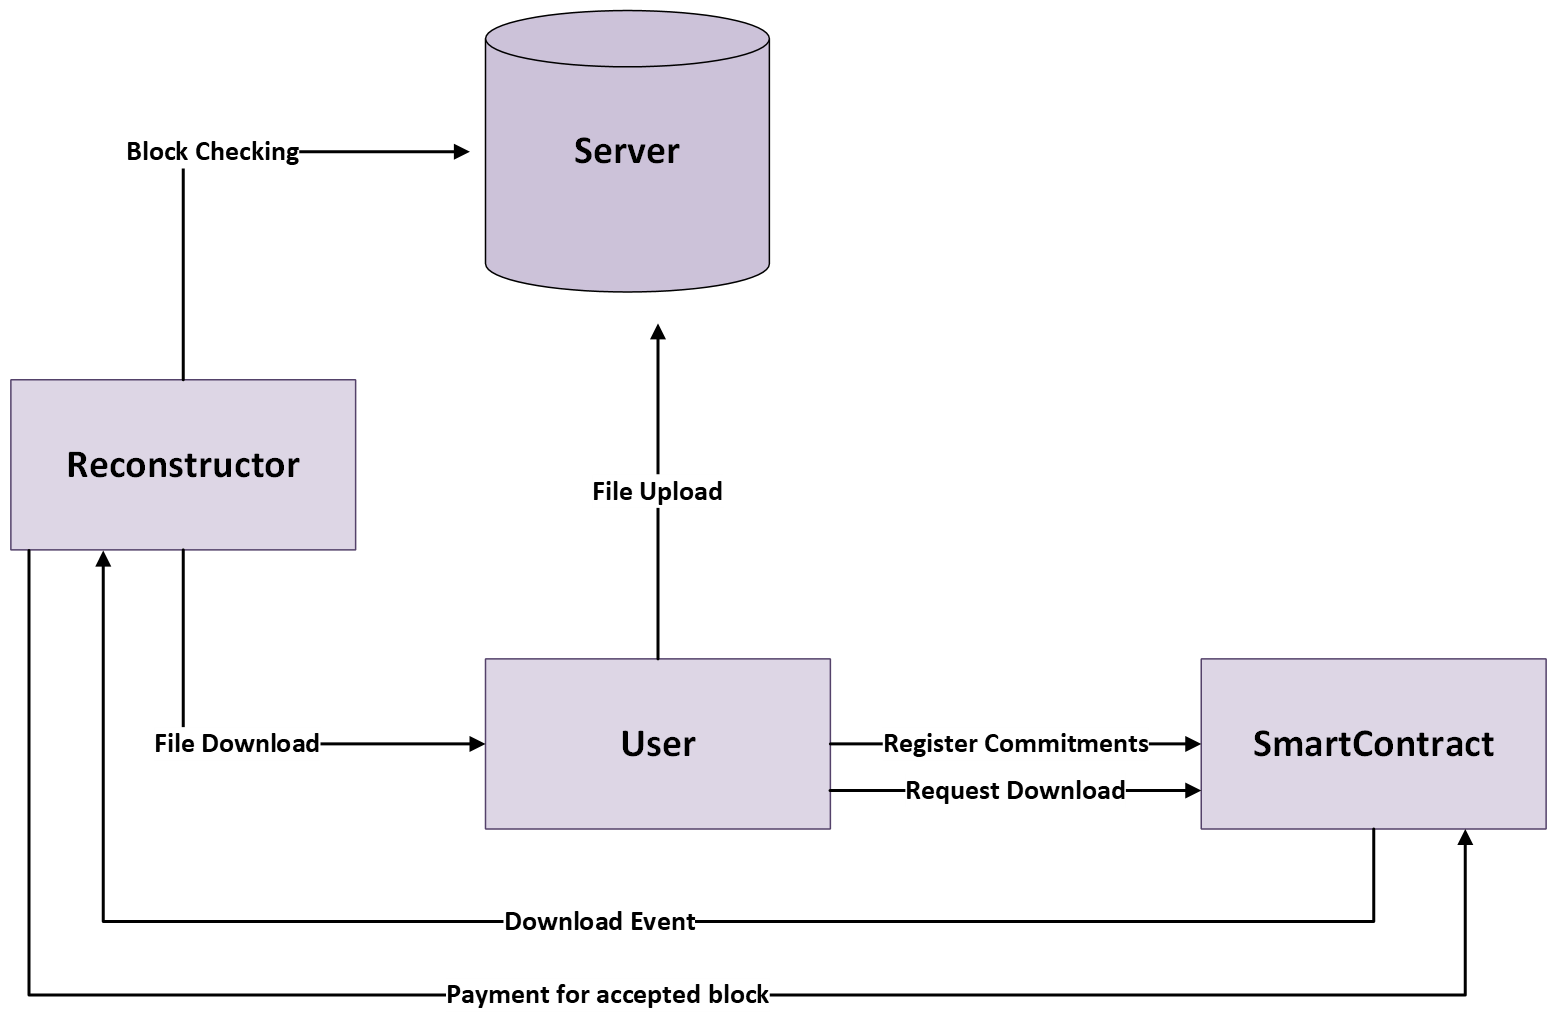
\includegraphics[width=\textwidth]{img/Hysail-Architecture-Proposed.png}
	\caption{Nova Arquitetura de HySail utilizando blockchain como meio de auditoria}
\end{figure}

